% Metódy inžinierskej práce

\documentclass[10pt,twoside,slovak,a4paper]{article}

\usepackage[slovak]{babel}
%\usepackage[T1]{fontenc}
\usepackage[IL2]{fontenc} % lepšia sadzba písmena Ľ než v T1
\usepackage[utf8]{inputenc}
\usepackage{graphicx}
\usepackage{dirtytalk}
\usepackage{url} % príkaz \url na formátovanie URL
\usepackage{hyperref} % odkazy v texte budú aktívne (pri niektorých triedach dokumentov spôsobuje posun textu)

\usepackage{cite}
%\usepackage{times}

\pagestyle{headings}

\title{Učenie sa pomocou hier\thanks{Semestrálny projekt v predmete Metódy inžinierskej práce, ak. rok 2022/23, vedenie: Ing. Zuzana Špitálová}} 

\author{Dominika Lukašáková\\[2pt]
	{\small Slovenská technická univerzita v Bratislave}\\
	{\small Fakulta informatiky a informačných technológií}\\
	{\small \texttt{xlukasakova@stuba.sk}}
	}

\date{\small 22. október 2022}



\begin{document}

\maketitle

\begin{abstract}
%\ldots
Tento článok je zameraný na učenie sa pomocou hier. Článok vysvetľuje pojem seriózne hry (časť~\ref{Vazne hry}), ako fungujú a aké prostriedky, nástroje a technológie na učenie využívajú (časť~\ref{Fungovanie}). Článok ďalej vysvetľuje ako môžu tieto hry vplývať na študentov (časť~\ref{Vplyv}), a to teda pozitívne, ale aj negatívne. Taktiež uvádza príklady v praxi (časť~\ref{Prax})- rôzne simulácie a videohry a oblasti v ktorých sa vážne hry využívajú. 
\end{abstract}



\section{Úvod}


Hry boli odjakživa atraktívne pre mladých ľudí, pretože slúžili ako únik od reality. Keď hovoríme o zábave na počítači, tak tým väčšinou myslíme počítačové hry alebo pozeranie filmov a videí. Pod pojmom „počítačové hry“ si vybavíme hlavne nezmyselné bojové hry, ktoré nemajú špeciálnu výchovnú a vzdelávaciu hodnotu, avšak hry, ktoré boli určené hlavne na zábavu, môžu prípadne aj vzdelávať. Napríklad, ak ide o použitie geometrických útvarov v hre ako Tetris, tak si hráči istým spôsobom precvičujú aj priestorové myslenie. Práve preto, by mali pedagógovia využiť túto skutočnosť vo svoj prospech. Vzdelávacie hry môžu byť účinnými nástrojmi na vzdelávanie, pretože prirodzene motivujú a poskytujú interaktívnu formu učenia, a tak povzbudzujú študentov byť aktívnymi účastníkmi vzdelávacieho procesu. 

\vspace{5mm} %5mm vertical space

\emph{\say{Motivácia je najdôležitejším faktorom, ktorý poháňa učenie. Keď motivácia zomrie, chuť na hranie sa zastaví a učenie zomrie.}} \cite{Gee}

\newpage

\section{Počítačové hry}


Téma „počítačové hry“ vždy vyvolala u rodičov a odborníkov veľký rozruch, a to zväčša negatívny. Počítačové hry majú však aj pozitívny význam:   

\begin{itemize}
\item Pomocou hier sa človek učí zaobchádzať s počítačovou technikou
\item Pomocou počítačových hier sa deti učia písať, počítať, logicky myslieť
\item Počítačové hry podporujú tiež záujem o programovanie a ďalší vývoj technológií
\end{itemize}


\vspace{5mm}

Rozdelenie hier...


\section{Vážne hry} \label{Vazne hry}


Popri hrách určených na zábavu existuje rozsiahla oblasť takzvaných „vážnych hier“ (anglicky „serious game“), kde sa herné technológie využívajú spravidla na osvojenie si nových poznatkov a zručností v rôznych oblastiach.

\vspace{5mm}

Viac popísané a vysvetlené...


\subsection{Princíp fungovania vzdelávacích hier} \label{Fungovanie}



Vážne hry úzko spolupracujú s kognitívnou vedou, keďže kognitívna veda sa zaoberá skúmaním ľudskej mysle, procesov vnímania, myslenia, rozhodovania, učenia a konania. Vážne hry teda zahŕňajú prvky niekoľkých kognitívnych zručností, ktoré sú priamo alebo nepriamo zapojené do procesu učenia. Patrí tam napríklad pozornosť a vizuálno-priestorové schopnosti, pamäť a motorické zručnosti. \cite{Ypsilanti}

\vspace{5mm} %5mm vertical space

Študenti majú často problém v chápaní a zapamätávaní si informácií, ktoré dostali mimo kontextu alebo príliš dlho predtým, ako ich mohli použiť. Avšak vážne hry toto nerobia. Celkovo vzaté, vážne hry umožňujú študentom uplatniť ich súčasné poznatky v digitálnom prostredí s cieľom osvojenia si nových zručností. \cite{Gee}


\subsection{Vplyv hier na študentov} \label{Vplyv}


Hra je jednou zo základných činností zvierat aj ľudí. Schopnosť hrať sa máme už od narodenia. Hra nás v detstve pripravuje na skutočný svet. Hrou sa rozvíja ľudská predstavivosť a je najjednoduchším spôsobom učenia. Hry prinášajú pocit uspokojenia, únik pred problémami dnešnej reality, radosť z víťazstva ale aj sklamanie pri prehre.  Tak ako všetko v živote, aj hry vplývajú na študentov pozitívne ale aj negatívne. V dnešnej dobe je na trhu množstvo hier, preto treba dávať veľký pozor pri ich výbere.

\vspace{5mm}
K pozitívnym vplyvom patrí: 

\begin{itemize}
\item prirodzená motivácia
\item získanie nových informácii
\item schopnosť samostatne sa rozhodovať
\item schopnosť riešiť problémy
\item osvojenie si nových zručností
\end{itemize}

\vspace{5mm}
K negatívnym vplyvom patrí: 

\begin{itemize}
\item strata schopnosti komunikácie s okolím
\item život v nereálnom vlastnom svete
\item agresívne správanie
\item neschopnosť riešiť bežné problémy
\item závislosť na hrách
\end{itemize}


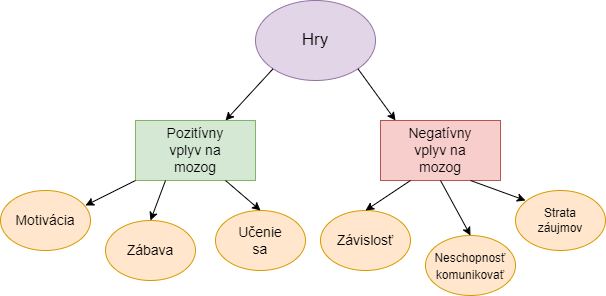
\includegraphics[scale=0.5]{vplyv_na_mozog.drawio.png}


\subsection{Príklady v praxi} \label{Prax}


\section{Záver}



%\acknowledgement{Ak niekomu chcete poďakovať\ldots}


% týmto sa generuje zoznam literatúry z obsahu súboru literatura.bib podľa toho, na čo sa v článku odkazujete
\bibliography{literatura}
\bibliographystyle{plain} % prípadne alpha, abbrv alebo hociktorý iný
\end{document}
